\section{The FSM Driver}
The proposal for controlling the car is a \emph{Finite State Machine}, which
enables a modular development, ideal for teamwork, and separates behaviors, reducing
the effort necessary to evolve a complete controller by breaking this problem into
evolving each state.

FSMs have been one of the favorite instruments f'or AI gaming, and they are present 
in many digital games~\cite{buckland2005}, due to characteristics as follows:

\begin{itemize}
	\item \textbf{Readiness}: a FSM is quickly and simply implemented, in almost every one of its forms.
	
	\item \textbf{Modularity}: debugging and refactoring a FSM becomes a catalyzed processe due to the abstraction of its
	structure, that is, its behavior can be divided into smaller, independent parts, which can be treated separately
	in a way that reduces the effort.
	
	\item \textbf{Low computational complexity}: a FSM would hardly ever require great amounts of processor time, and
	that is because its operation mainly follows but hard-coded rules.
	
	\item \textbf{Intuitive behavior}: analyzing a FSM is an easy process because human minds are often used to
	categorizing situations and conditions of conduct. This characteristic is both a good employment for debugging in
	real time and for turning the pilot's behavior simple enough so that a common person, i.e. non-programmer, could
	identify mistakes and spectate a race understanding the development of the pilot.
	
	\item \textbf{Flexibility}: a fundamental quirk of a FSM, one which makes the process of expanding the scope of the
	structure easier in a level hardly other choice of method would provide. If a new situation occurs, one that was
	not foreseen by the states defined and also one that could not be inserted in any of them, the mere creation of a
	new state would solve the matter, in about no time and almost without interference in the other parts of the whole.
\end{itemize}

	The division of states for the FSMDriver itself are in agreement with the advantages of a FSM, meaning that the choice of
	which states to be used relied on the human intuition of the development of a car in operation. The states designed are:

\begin{figure}[!t]
	\centering
	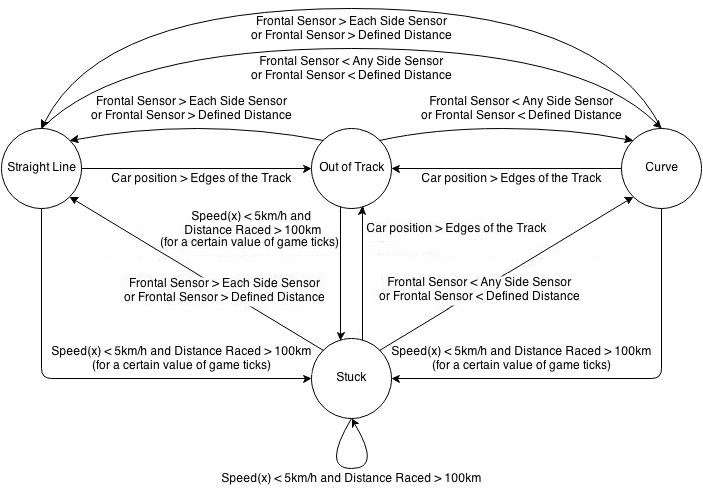
\includegraphics[width=3in]{StatesDiagram}
	\caption{State transition diagram.}
	\label{fig_sim}
\end{figure}

\begin{itemize}
	\item \textbf{Straight line}: The state in which the pilot commands the car to full throttle and maximum 
	speed/acceleration ahead, and occurs when the car is located in a situation that sees no turning nearby;
	
	\item \textbf{Curve}: A curve can be assumed as a critical event in a race once it take the car's controller
	to act almost abruptaly in order to continue the race, these actions not always are the most appropriate, it
	may be enough to the car be overtaken by other competitors. The way to handle obliqual tracks was based 
	on the position of the car and the angle between the direction of the car axis and the track axis direction, 
	values adquired by two sensors that affect the actuators: steering, gear and clutch. It is focused on the 
	steering of the car, that is, changing its direction of movement in order to keep it inside the delimitations 
	of the proper racing space and also to avoid crashing the car into an obstacle;
	
	\item \textbf{Out of track}: When the previous states fail to prevent the car from entering an undesired situation
	such as going outside of the track, where conditions such as friction are much worse for the car than inside the
	track, this state takes control of the car and tries to return it to the race;
	
	\item \textbf{Stuck}: In a worst case scenario, when the car is barely moving, drastic measures need to be taken,
	such as reversing the car and steering it out of an obstacle. The appearence of such events reduce largely the
	performance of the pilot in the race.
\end{itemize}

	In other words, the pilot will encounter four situations in a race, two of them are desired, whereas the other two are 
	emergency actions. While the car is either on a \emph{straight line} or on a \emph{curve}, the behavior is normal; 
	but when the criteria defined to manipulate the pilot into entering those states fails to keep it racing, and the car 
	goes \emph{outside of the track} or gets \emph{stuck}, the car encounters troubles and loses performance. That is why
	the accurate definition of the requirements the pilot has to fulfill to be in each of these states needs to be thought 
	thoroughly for good and competitive results.

	Each state of the FSMDriver uses specific parameters for defining its behavior. 
	There is a transition function that uses specific (\emph{constant}) parameters
	to decide when the \emph{current state} needs to be changed (and which state to
	change to). This function mainly uses four constants:
	\begin{itemize}
		\item \textbf{MSD}, the maximum distance the frontal sensor can reach when in full speed
		(\textbf{M}aximum \textbf{S}peed \textbf{D}istance);
		\item \textbf{LE}, track position value that indicates the left boundary of the proper racing
		space (\textbf{L}eft \textbf{E}dge);
		\item \textbf{RE}, track position value that indicates the right boundary of the proper racing
		space (\textbf{R}ight \textbf{E}dge);
		\item \textbf{ST}, number of ticks required by the controller for it to declare being stuck
		(\textbf{S}tuck \textbf{T}icks).
	\end{itemize}
	
	The procedure of analysis to check the current state of the car in the race is
	based on the following: to be \emph{outside of track} the car needs to be out of
	the range defined between \emph{LE} and \emph{RE}, which are modularized values
	that relate to the edges of the track. If the car is inside those values, than it
	is correctly inside the track and can be either on a \emph{straight line},
	when the frontal distance sensor is bigger than the \emph{MSD} or when this same
	sensor points to a bigger value than the adjacent side sensors, or on a
	\emph{curve}, when none of these two requirements is fulfilled. Before all of
	these conditions are checked, which happens at every game tick, the car goes through
	a procedure of verification on the \emph{stuck} state, that is, if it is at a defined
	low speed and is not on the beginning of the track where it is acceptable, the game
	ticks are accumulated until the defined value of maximum ticks in stuck conditions
	\emph{ST} is reached, indicating that the car went stuck. Given this behavior, the
	\emph{transition} function was implemented, and as it is the part of the code that
	has less variables for perfomance-improvement analysis, it was submitted for
	exaustive testing as a first attempt to evolve parameters inside the controller.
